\subsection{Resultados Complementarios de Ordenamiento}

En la Figura~\ref{fig:sorting_descendente} se detalla el comportamiento temporal y el consumo de memoria para secuencias ordenadas de manera descendente. Se observa cómo el algoritmo PatienceSort experimenta su peor escenario en consumo de memoria auxiliar ($\approx 500$ MB para $N = 10^7$), ya que cada elemento nuevo genera una pila independiente en el sistema, elevando la dispersión en el \textit{heap}.

\begin{figure}[htbp]
    \centering
    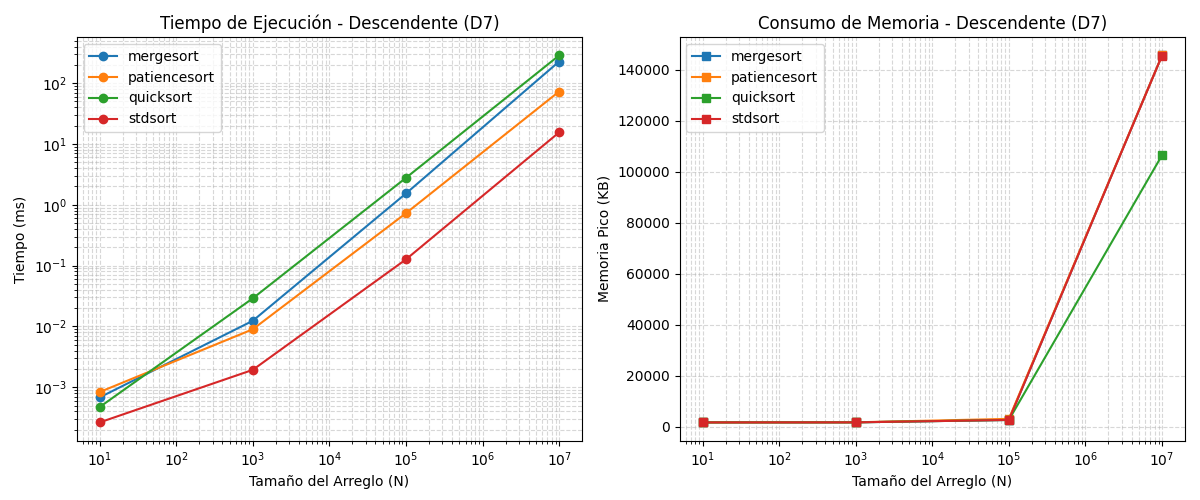
\includegraphics[width=0.75\textwidth]{../code/sorting/data/plots/sorting_descendente_D7.png}
    \caption{Tiempo de ejecución y memoria en arreglos descendentes ($D7$).}
    \label{fig:sorting_descendente}
\end{figure}

\subsection{Comportamiento en Matrices Diagonales}

La Figura~\ref{fig:matrix_diagonal} ilustra el rendimiento de Naive y Strassen sobre matrices con coeficientes no nulos restringidos a la diagonal principal. Los tiempos son análogos a los de matrices densas, confirmando experimentalmente la ausencia de optimizaciones estructurales o podas condicionales en el código evaluado.

\begin{figure}[htbp]
    \centering
    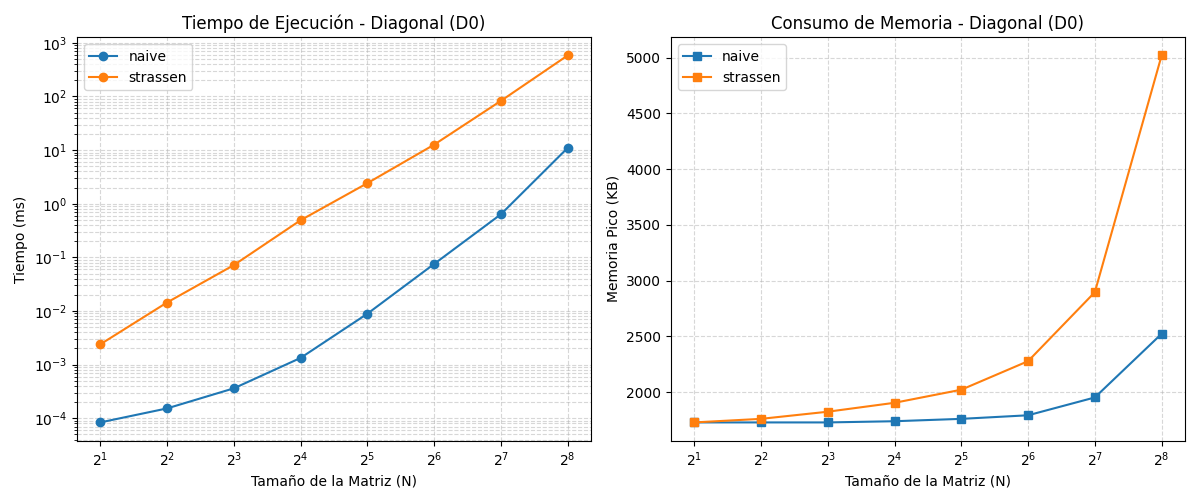
\includegraphics[width=0.75\textwidth]{../code/matrix_multiplication/data/plots/matrix_diagonal_D0.png}
    \caption{Rendimiento en matrices diagonales con dominio $D0$.}
    \label{fig:matrix_diagonal}
\end{figure}
 